\paragraph{arithmetic\_extension}

To understand the design principle of this Gate, we must first understand \href{https://en.wikipedia.org/wiki/Field_extension#Extension_field}{Field extension}. 


Taking Plonky2's GoldilocksField as an example, we give the extension field elements under quadratic, quartic, and quintic extensions respectively in \figref{fig:goldilocksfield-extension}.

\begin{figure}[!ht]
    \centering
    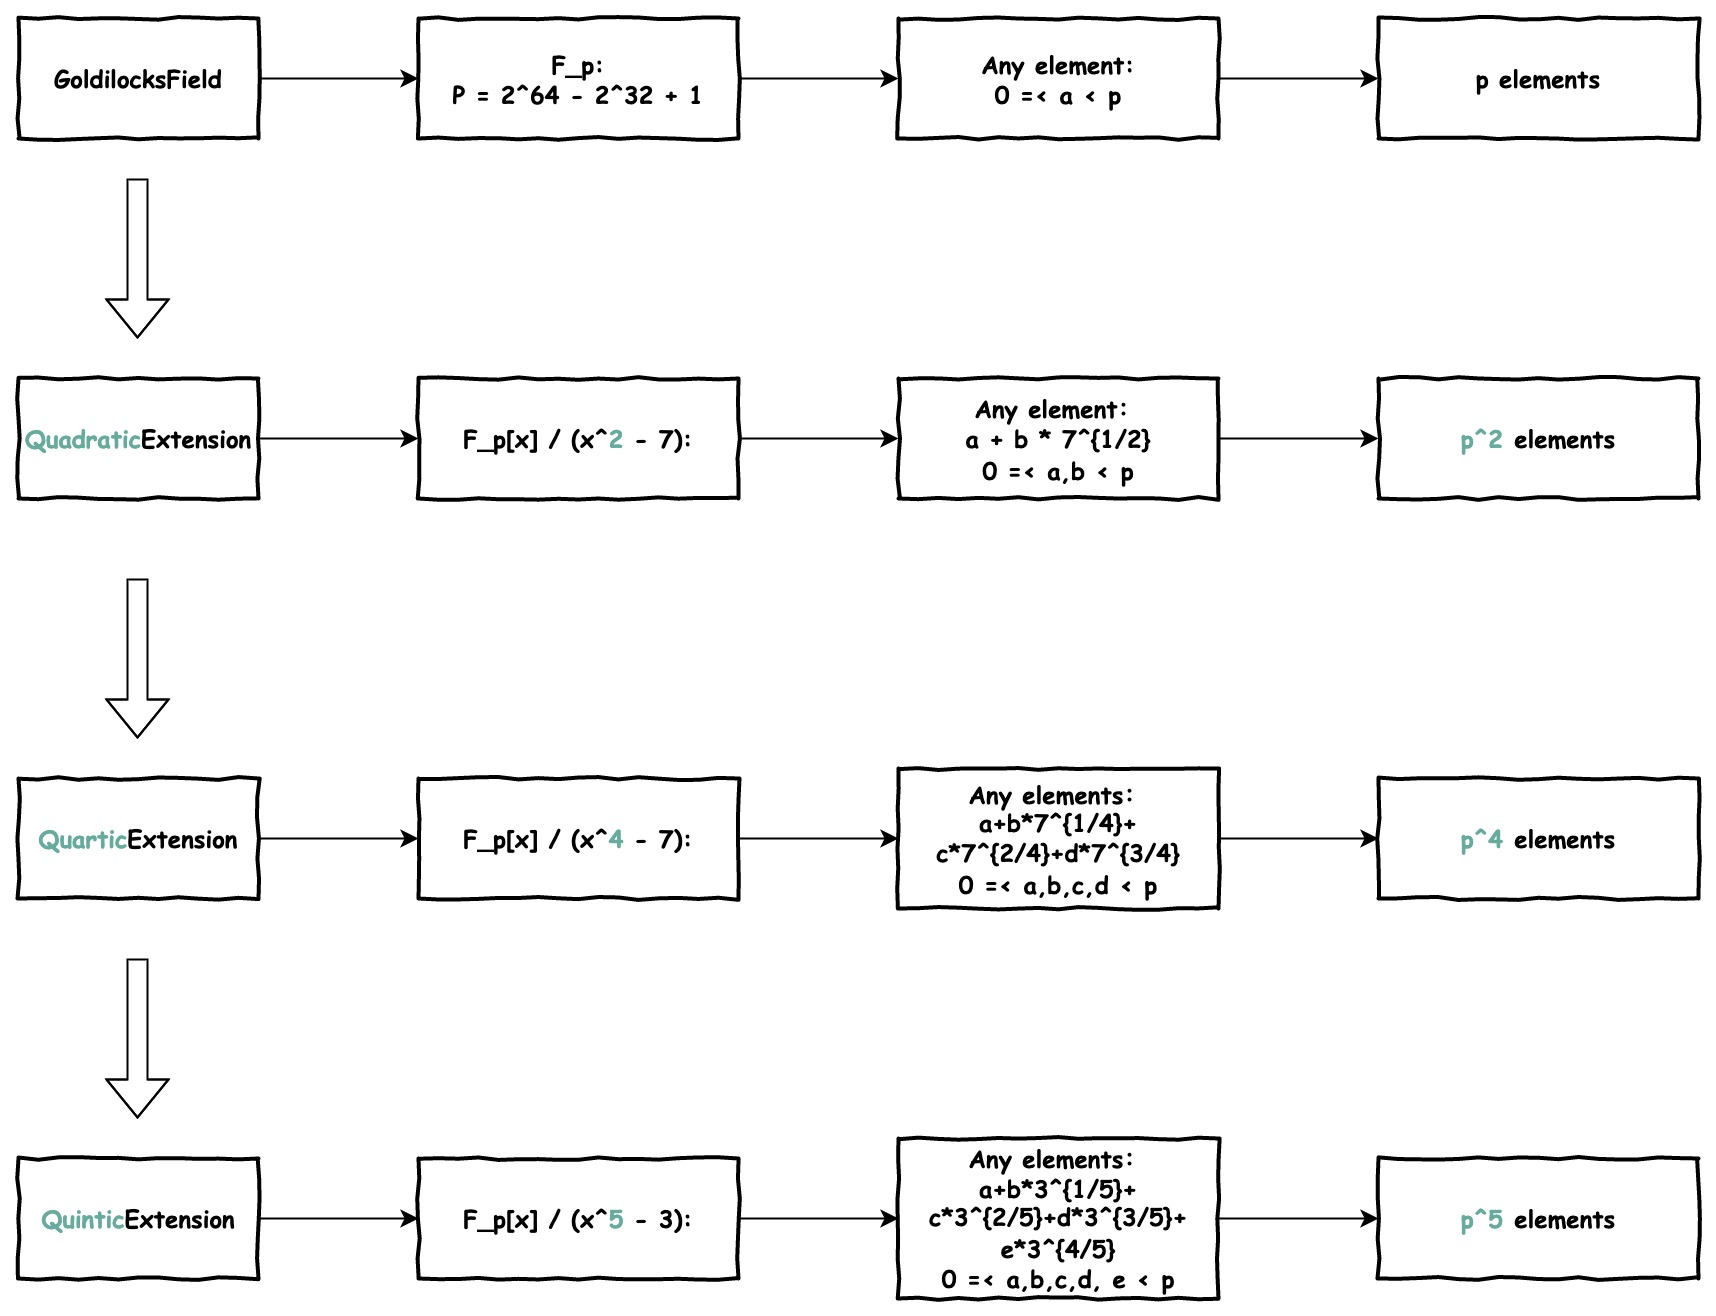
\includegraphics[width=0.6\textwidth]{gates/arthmetic_extension_ext.jpeg}
    \caption{GoldilocksField Extension}
    \label{fig:goldilocksfield-extension}
\end{figure}

It is easy to see that for QuadraticExtension Field, the elements on its domain take the form $a+b\sqrt{7}, \ a,b \in F_p$.
It can be seen that on the quadratic extension domain, there are $p^2$ elements and the original domain is a subset of the quadratic extension domain.

ArithmeticExtensionGate is also a gate that can perform a weighted multiply-add, i.e.
\[ \text{res} = \text{cons\_0} \times \text{mul\_0} \times \text{mul\_1} + \text{cons\_1} \times \text{add} \]
The elements of the QuadraticExtension Field are represented in the form $[a, b]$, so the Gate design for arithmetic\_extension has the following form:

The structure of the gate is shown in \figref{fig:arthmetic-extension}.
\begin{figure}[!ht]
    \centering
    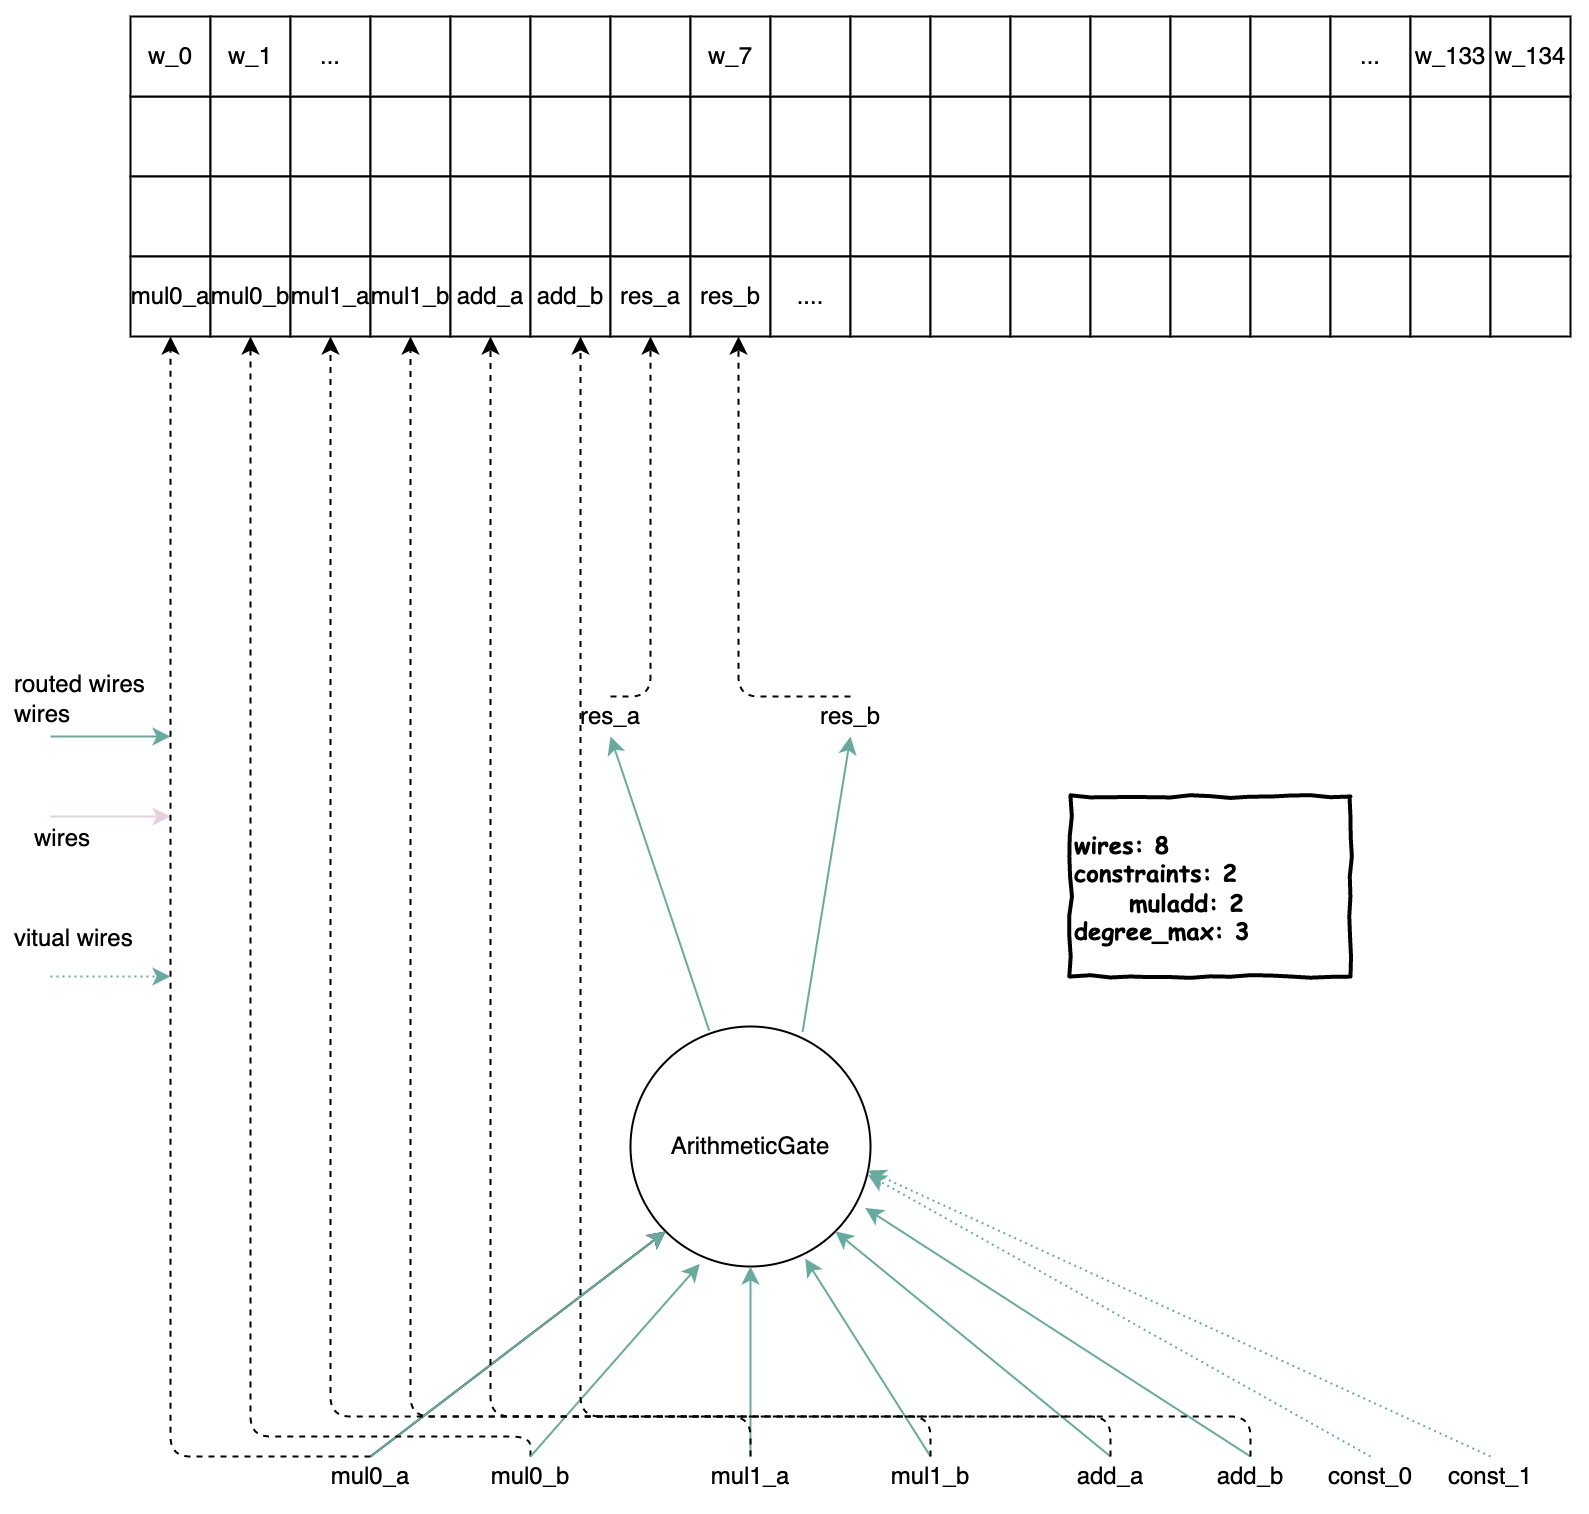
\includegraphics[width=0.6\textwidth]{gates/arthmetic_extension.jpeg}
    \caption{ArithmeticExtensionGate}
    \label{fig:arthmetic-extension}
\end{figure}

There's only one constraint per operation, and the degree is 3.
